\chapter{SQL - Structured Query Language}
SQL è un linguaggio per la definizione e la manipolazione dei dati
in database relazionali adottato da molti DBMS. \\
Ci sono diverse versioni, la prima versione ufficiale risale al 1986.
Poi sono state rilasciate altre versioni come SQL-89, SQL-2, SQL-3\dots\\
Noi faremo riferimento principalmente a SQL-2. Questa versione è ricca e complessa,
tanto che nessun sistema commerciale lo implementa in maniera completa.\\
Esistono 3 livelli di conformità:
\begin{itemize}
  \item Entry level: molto simile a SQL-89
  \item Intermediate level: versione che soddisfa le esigenze di mercato
  \item Full level: versione completa anche delle funzioni avanzate che non sono realizzate
        in alcun DBMS
\end{itemize}
La maggior parte dei database è conforme solo all'entry level.\\
Alcune famose implementazioni di SQL sono:
\begin{itemize}
  \item ORACLE
  \item DB2 (IBM)
  \item Access (Microsoft)
  \item MSSQL server (Microsoft)
  \item MySQL
  \item Firebird
\end{itemize}
\section{Confronto con Algebra Relazionale e Istruzioni principali}
\subsection{SQL e Algebra Relazionale}
SQL è relazionalmente completo: ogni espressione logica può essere tradotta in SQL.
Viene adottata la logica dei 3 valori (T, F, U) dell'Algebra relazionale (U = Unknown).\\
Il modello dati di SQL è basato su tabelle anzichè relazioni (possono essere presenti righe duplicate).\\
SQL è computazionalmente completo, ha istruzioni di controllo.\\
\paragraph*{Logica a 3 valori} Logica che utilizza:
\begin{itemize}
  \item True
  \item False
  \item Unknown
\end{itemize}
Che segue la seguente tabella di verità
\begin{table}[h]
  \centering
  \caption{SQL Three-Value Logic Truth Table}
  \begin{tabular}{|c|c|c|c|}
    \hline
    \textbf{Value 1} & \textbf{Value 2} & \textbf{AND} & \textbf{OR} \\
    \hline
    TRUE             & TRUE             & TRUE         & TRUE        \\
    \hline
    TRUE             & FALSE            & FALSE        & TRUE        \\
    \hline
    TRUE             & UNKNOWN          & UNKNOWN      & TRUE        \\
    \hline
    FALSE            & TRUE             & FALSE        & TRUE        \\
    \hline
    FALSE            & FALSE            & FALSE        & FALSE       \\
    \hline
    FALSE            & UNKNOWN          & FALSE        & UNKNOWN     \\
    \hline
    UNKNOWN          & TRUE             & UNKNOWN      & TRUE        \\
    \hline
    UNKNOWN          & FALSE            & FALSE        & UNKNOWN     \\
    \hline
    UNKNOWN          & UNKNOWN          & UNKNOWN      & UNKNOWN     \\
    \hline
  \end{tabular}
\end{table}

\subsection{Istruzioni principali DDL}
Operazioni di definizione schema e modifica
\begin{itemize}
  \item CREATE - Definisce database, tabelle, domini, viste, vincoli e autorizzazioni
  \item ALTER - Modifica attributi e vincoli
  \item DROP - Elimina database e tabelle
\end{itemize}
\subsection{Istruzioni principali DML}
Operazione di interrogazione: SELECT. Formula Query come nell'AR o anche
richieste più elaborate.\\
\subsection*{Aggiornamento}
\begin{itemize}
  \item INSERT - Inserisce nuove tuple nelle tabelle
  \item DELETE - Elmina tuple nelle tabelle
  \item UPDATE - Modifica tuple
\end{itemize}
Queste ultime possono basarsi sul risultato di una query.
\subsection{SQL è dichiarativo}
Essendo principalmente dichiarativo non possiamo scegliere l'ordine in cui
avvengono le operazioni è necessario attenersi alla struttura sintattica delle
istruzioni.
\subsection{Notazione SQL}
\begin{itemize}
  \item Termini del linguaggio in MAIUSCOLO
  \item Termini variabili (specificati dall'utente) in minuscolo
  \item <x> usate per isolare un termine x
  \item [x] indicano che il parametro è opzionale
  \item | seprara opzioni alternative
\end{itemize}

\subsection{Primo esempio di Query}
\begin{lstlisting}[language=SQL]
  SELECT ListaAttributi
  FROM ListaTabelle
  [WHERE Condizione]
\end{lstlisting}
Dove SELECT e FROM sono obbligatori, mentre WHERE è opzionale (in realtà c'è praticamente
sempre in quanto serve per filtrare i risultati).\\
\section{SQL-DDL}
Uno schema di base di dati è una collezione di oggetti: domini, tabelle,
asserzioni, viste, privilegi. La sintassi è la seguente:
\begin{lstlisting}[language=SQL]
  CREATE SCHEMA 
    [Nome Schema]
    [[AUTHORIZATION] Autorizzazione]
    {DefinizioneElementoSchema}
\end{lstlisting}
Nome schema se omesso indica l'utente che ha lanciato il comando, mentre
autorizzazione è il proprietrio dello schema (utente che lo ha definito).\\
\subsection{Tabelle}
Tramite CREATE TABLE si definisce una tabella. Una tabella non è altro che uno
schema di relazione, con CREATE viene creata un'istanza vuota.
\begin{lstlisting}[language=SQL]
  CREATE TABLE NomeTabella
    (NomeAttributo1 TipoDominio1 [Valore di Default] [Vincolo1],
    NomeAttributo2 TipoDominio2 [Valore di Default] [Vincolo2],
    ...
    [AltriVincoli])
\end{lstlisting}
In questo ambito parleremo di tabelle e non di relazioni, e di righe e non di tuple,
perchè rispetto al modello relazionale possiamo avere righe duplicate.\\
Qui di seguito un esempio reale di definizione di tabella:
\begin{lstlisting}[language=SQL]
  CREATE TABLE Impiegato(
    Matricola CHAR(6) PRIMARY KEY,
    Nome CHAR(20) NOT NULL,
    Cognome CHAR(20) NOT NULL,
    Dipart CHAR(15),
    Stipendio NUMERIC(9) DEFAULT 0,
    FOREIGN KEY(Dipart) REFERENCES
    Dipartimento(NomeDip),
    UNIQUE (Cognome,Nome)
)
\end{lstlisting}
\subsection{Definizione dei Dati: I Domini}
I domini specificano i vlori ammessi da ciascun attributo. SQL ha 
6 domini elementari predefiniti:
\begin{itemize}
  \item Carattere- VARCHAR - Stringa di lunghezza variabile tra 0 e n
  \item Numerico Esatto - INTEGER, SMALLINT, NUMERIC
  \item Numerico Approssimato - FLOAT, REAL, DOUBLE PRECISION
  \item Data/Ora TIMESTAMP, DATE, TIME
  \item Intervallo Temporale
  \item Bit (SQL-2) - BOOLEAN (SQL-3) - con dominio 0,1
\end{itemize}
Bit è stato poi eliminato e sostituito parzialmente da BOOLEAN in SQL-3\\
L'utente pu definire dei domini custom (semplici, ma riutilizzabili).\\
\paragraph*{BLOB, CLOB} sono oggetti di grandi dimensioni, costituiti da binari (BLOB)
o caratteri (CLOB), vengono memorizzati in maniera differente dagli altri dati e sono usati per memorizzare
informazioni non strutturate (immagini, video, testi\dots).\\
\subsection{Il tipo Bit}
Utilizzato spesso per definire se è presente o meno una certa proprietà, dato
che si tratta di un BOOLEAN.
\subsection{Carattere}
Si indica:
\begin{lstlisting}[language=SQL]
  CHAR(n) - Stringa di lunghezza fissa n
  VARCHAR(n) - Stringa di lunghezza variabile tra 0 e n
\end{lstlisting}
\subsection{Numerici Esatti}
Rappresentano numeri interi o numeri decimali in virgola fissa (con un numero prefissato
di decimali, come per i valori monetari). Precisionè il numero di cifre significative,
scala il numero di cifre dopo la virgola.\\
\begin{itemize}
  \item INTEGER/SMALLINT rappresentano valori interi - La precisione varia a seconda della
  specifica implementazione di SQL, SMALLINT richiede meno spazio di memorizzazione
  \item NUMERIC/DECIMAL rappresentano valori decimali - La differenza fra questi due è che
  il primo deve essere implementato esattamente con la precisione richiesta, mentre il secondo
  può avere una precisione maggiore.
\end{itemize}
\subsection{Numerici Approssimati}
Sono utili per rappresentare valori reali approssimati, ad esempio grandezze
fisiche (rappresentazione in virgola mobile, in cui a ciascun numero corrisponde
una coppia di valori: mantissa e esponente).\\
REAL e DOUBLE PRECISION rappresentano valori a singola/doppia precisione in virgola
mobile. FLOAT permette di richiedere la precisione che si desidera.
\subsection{Data e Ora}
Permettono di descrivere informazioni temporali, rappresentando istanti di tempo:
\begin{itemize}
  \item DATE rappresenta le date espresse come anno (4 cifre), mese (2 cifre) e giorno (2 cifre)
  - DATE 'yyyy-mm-dd'
  \item TIME [WITH TIME ZONE] rappresenta l'ora del giorno, espressa come ora (2 cifre), 
  minuti (2 cifre) e secondi (2 cifre)
  \item TIMESTAMP
\end{itemize}
Ciascuno di questi domini è strutturato e decomponibile in un insieme di campi 
(anno, mese, giorno, ora, minuti, secondi).
\subsection{Intervalli temporali}
Permette di rappresentare intervalli di tempo come durate di eventi.\\
INTERVAL rappresenta una durata temporale, esistono interval ani e mesi, oppure
giorni e ore, ma non mesi e giorni poichè i mesi non hanno tutti lo stesso numero di
giorni.
\subsection{CLOB e BLOB}
Permettono di includere nel database oggetti molto grandi (come dati multimediali).
Sono implementati come valore e non possono essere usati come criterio di selezione per le
query.
\subsection{Domini definiti dall'utente}
\begin{lstlisting}[language=SQL]
  CREATE DOMAIN Voto AS SMALLINT
    DEFAULT 0
    CHECK (VALUE >= 18 AND VALUE <= 30)
\end{lstlisting}
Possono mettere vincoli puù o meno utili.\\
Al contrario dei meccanismi di definizione dei tipi nei linguaggi di programmazione,
SQL-2 non mette a disposizione dei costruttori di dominio come record o array. Questa 
caratteristica deriva dal modello relazionale dei dati il quale richiede che ogni
attributo sia definito su un dominio elementare.
\subsection{Valori di Deafult}
Definiscono il valore che deve assumere l'attributo quando non viene specificato 
un valore durante l'inserimento di una tupla.\\
DEFAULT $<$ ValoreGenerico | user | null $>$
\begin{itemize}
  \item ValoreGenerico rappresenta un valore compatibile con il dominio,
  rappresentato come una costante o come un’espressione.
  \item user è l’identificativo dell’utente che effettua il comando di
  aggiornamento della tabella.
  \item null è il valore di DEFAULT di base.
\end{itemize}
\subsection{Il valore NULL}
\'E un valore polimorfico che appartiene a tutti i domini con il significato di valore
non noto.
\begin{itemize}
  \item Il valore esiste ma non è noto al database
  \item Il valore è inapplicabile (es. numero patente per minorenni)
  \item Non si sa se il valore è inapplicabile o meno (es. numero patente per un maggiorenne)
\end{itemize}
\subsection{Vincoli di Integrità}
Un vincolo è una regola che specifica delle condizioni sui valori di un elemento
dello schema del database. Un vincolo può essere associato ad una tabella, ad un attributo,
ad un dominio.
\begin{itemize}
  \item Vincoli Intrarelazionali - Proprietà sempre valida all'interno di una relazione
  \item Vincoli Interrelazionali - Proprietà sempre valida tra relazioni diverse
\end{itemize}
\paragraph*{Sintassi}
\begin{itemize}
  \item NOT NULL - Valore non nullo
  \item UNIQUE - Valore unico
  \item PRIMARY KEY - Chiave primaria
  \item CHECK - Definisce condizioni complesse (sia intra che inter relazionali)
\end{itemize}
\paragraph*{Esempio}
\begin{lstlisting}[language=SQL]
  Nome CHAR(20) NOT NULL
  Cognome CHAR(20) NOT NULL 
  UNIQUE (Nome, Cognome)
\end{lstlisting}
NOT NULL su Nome e Cognome è un vincolo intrarelazionale,
UNIQUE è Interrelazionale (non posso avere istanze uguali ripetute)
\subsection{Chiave}
Insieme di attributi che identificano univocamente una tupla all'interno di
una relazione. Il vincolo PRIMARY KEY può essere definito una volta sola all'interno
della relazione (implicitamente NOT NULL e UNIQUE).
\paragraph*{Eccezioni} Il valore NULL può comparire su diverse righe senza violare
il vincolo.
\subsection*{CHECK e FOREING KEY}
Utilizzato per definire vincoli complessi, sia intrarelazionali che interrelazionali.
\begin{lstlisting}[language=SQL]
  CREATE TABLE Studente (
    CREATE DOMAIN Voto AS SMALLINT
    DEFAULT 0
    CHECK (Voto>=18 AND VOTO<=30)
  )
\end{lstlisting}
Per quanto riguarda invece i vincoli interrelazionali, si utilizza FOREIGN KEY e
REFERENCES.\\
\paragraph*{FOREIGN KEY} Un vincolo di intergrità referenziale ("FOREIGN KEY") 
fra gli attributi X di una relazione $R_1$ e un'altra relazione $R_2$ impone ai valori su X,
in $R_1$ di comparire come vlaori della chiave primaria di $R_2$.\\
Un vincolo di intergrità referenzialie fra gli attributi $X={A_1, A_2,...}$ di una
tabella figlio interna e un'altra tabella padre esterna impone ai valori degli attributi X
nella tabella Figlio di comparire come valori della chiave primaria nella Tabella Padre.\\
Alcuni attributi della tabella figlio sono definiti come FOREIGN KEY e si devono riferire (REFERENCES)
ad alcuni attributi della tabella padre che costituiscono una chiave (devono essere UNIQUE e NOT NULL, oppure
PRIMARY KEY).\\
I valori contenuti nella FOREIGN KEY devono essere sempre presenti nella tabella
padre.\\
La tabella Figlio viene anche definita \textbf{interna}, mentre quella Padre \textbf{esterna}.\\
\paragraph*{Due sintassi} 
\begin{enumerate}
  \item Nella parte di definizione degli attributi con il costrutto sintattico
  REFERENCES
  \begin{lstlisting}
    AttrFiglio CHAR(3) REFERENCES TabellaPadre(AttrPadre)
  \end{lstlisting}
  \item Oppure dopo le definizione degli attributi con i costrutti FOREIGN KEY e REFERENCES
  \begin{lstlisting}
    FOREIGN KEY (AttrFiglio) REFERENCES TabellaPadre(AttrPadre)
  \end{lstlisting}
\end{enumerate}
Quando si hanno più attributi da riferire si utilizza sempre FOREIGN KEY e REFERENCES, se si
omettono gli attributi destinazione, vengono assunti quelli della chiave primaria.
\subsection{Aggiornamenti e Violazioni}
Se viene eseguita un'operazione di aggiornamento che viola un vincolo di integrità referenziale
la base di dati diventa non valida, per questo sono definite un insieme di politiche
per evitare che questo accada. Per i vincoli di integrità SQL permette di
scegliere delle reazioni da adottare in caso di violazioni, tali politiche vanno
dichiarate nella dichiarazione DDL dello schema.\\
Si possono introdurre violazioni operando sulle righe della tabella padre (esterna) o sulle righe
della tabella efiglio (interna)
\paragraph*{Modifiche Tabella Figlio}
\begin{itemize}
  \item Inserimento nuova riga
  \item Modifica della FOREIGN KEY
\end{itemize}
Non venogno proposte delle reazioni, le operazioni vengono rifiutate
\paragraph*{Tabella Padre}
\begin{itemize}
  \item Cancellazione riga
  \item Modifica dell'attributo riferito
\end{itemize}
Vengono proposte diverse reazioni:
\begin{itemize}
  \item CASCADE - L'operazione modifica/cancellazione viene propagata alla tabella figlio (o tabella interna)
  \item SET NULL - NULL nella tabella figlio in entrambi i casi
  \item SET DEFAULT - default nella tabella figlio in entrambi i casi
  \item NO ACTION - rifiutata in entrambi i casi
\end{itemize}
Le politiche di reazione possono essere definite in modo diverso per eventi di modifica/cancellazione
\begin{lstlisting}[language=SQL]
  Dipart CHARACTER(15) REFERENCES Dipartimento(NomeDip)
    ON DELETE SET NULL
    ON UPDATE CASCADE
\end{lstlisting}
Con CASCADE in pratica se effettuo una cancellazione cancello anche tutte le relazioni legati a quel valore,
con NULL invece pongo a NULL la FOREIGN KEY, ma mentengo gli altri valori.
\'E possibile assegnare un nome a questi vincoli, per rendere più chiaro il codice e rendere
quindi più semplice il debugging e la scrittura della documentazione.
\paragraph*{Sintassi nome vincoli}
\begin{lstlisting}[language=SQL]
  Stipendio INTEGER CONSTRAINT StipendioPositivo
  CHECK (Stipendio > 0),
  ...
  CONSTRAINT ForeignKeySedi
  FOREIGN KEY (Sede) REFERENCES Sedi
\end{lstlisting}

\section{Modifiche degli schemi}
Necessarie per garantire l'evoluzione della base di dati a fronte di nuove esigenze.\\
Ci sono 2 comandi SQL appositi:
\begin{itemize}
  \item ALTER - Modifica oggetti
  \item DROP - Cancella oggetti dallo schema
\end{itemize}
\subsection{ALTER}
\begin{itemize}
  \item ALTER DOMAIN - modifica domini (default, vincoli)
  \item ALTER TABLE - modifica tabelle
\end{itemize}
Attenzione: Quando si definisce un nuovo vincolo deve essere soddisfatto dalla istanza 
presente, altrimenti viene rifiutato.
\paragraph*{Modifiche degli schemi - DROP}
\begin{itemize}
  \item DROP DOMAIN - cancellazione del dominio (attributo)
  \item DROP TABLE - cancellazione della tabella
\end{itemize}
\paragraph*{Opzioni}
\begin{itemize}
  \item RESTRICT - Un oggetto (dominio, tabella) non è rimosso se non è vuoto
  \item CASCADE - viene rimosso l'oggetto e tutto ciò che è coinvolto
  nella definizione dell'oggetto
\end{itemize}
\paragraph*{Sintassi ALTER}
\begin{lstlisting}[language=SQL]
  ALTER DOMAIN NomeDominio <
    SET DEFAULT ValoreDefault|
    DROP DEFAULT|
    ADD CONSTRAINT DefVincolo |
    DROP CONSTRAINT NomeVincolo >
\end{lstlisting}
Esempio ALTER su tabella
\begin{lstlisting}[language=SQL]
  ALTER TABLE NomeTabella <
    ALTER COLUMN NomeAttributo<
      SET DEFAULTNuovoDefault |
      DROP DEFAULT> |
    DROP COLUMN NomeAttributo |
    ADD COLUMN DefAttributo |
    DROP CONSTRAINTNomeVincolo
    ADD CONSTRAINTDefVincolo >
\end{lstlisting}
\paragraph*{Sintassi DROP}
\begin{lstlisting}[language=SQL]
  DROP <schema, domain, table, view, ...> NomeElemento
    [RESTRICT | CASCADE]
\end{lstlisting}
\begin{itemize}
  \item RESTRICT - Impedisce drop se gli oggetti comprendono istanze non vuote
  \item CASCADE - Applica drop agli oggetti collegati, Potenziale pericolosa reazione
  a catena
\end{itemize}
\subsection{Cataloghi relazionali}
Il catalogo contiene il dizionario dei dati (data dictionary) ovvero la descrizione
della struttura dei dati contenuti nel database. Anche questa descrizione di dati (metadati)
è rappresentata tramite una struttura relazionale.\\
SQL-2 Organizza il catalogo su due livelli:
\begin{itemize}
  \item Definition\_Schema (composto da tabelle che descrivono tutte le strutture della
  base di dati)
  \item Information\_Schema (composto da viste che costituiscono l'interfaccia verso 
  il dizionario dei dati)
\end{itemize}

\section{Interrogazioni SQL - Query}
Le interrogazioni avvengono usando l'istruzione SELECT
\begin{lstlisting}[language=SQL]
  SELECT ListaAttributi
  FROM ListaTabelle
  [ WHERE Condizione ]
\end{lstlisting}
\begin{itemize}
  \item SELECT indica quali attributi vogliamo nel risultato
  \item FROM indica le tabelle da cui estrarre i dati
  \item WHERE indica che condizioni devono essere soddisfatte
\end{itemize}
SELECT non significa selezione, sceglie le colonne output della query.\\
FROM se vengono indicate più tabelle si effettua il loro prodotto cartesiano, 
salvo diversamente specificato (es. JOIN).\\
\subsection{Istruzione AS}
Si possono fare ridenominazioni su attributi e anche su relazioni con la clausola AS, 
molto utile per evitare di scrivere ogni volta l'attributo o la tabella per esteso
(specialmente se i nomi sono lunghi).\\
\begin{lstlisting}[language=SQL]
  SELECT AttrEspr [[AS] Alias]{,AttrEspr [[AS] Alias]}
  FROM Tabella [[AS] Alias]{,Tabella [[AS] Alias]}
  [WHERE Condizione]
\end{lstlisting}
Esempio pratico:
\begin{lstlisting}[language=SQL]
  SELECT Nome AS N, Stipendio AS Salario
  FROM Dipendente AS Dip
  WHERE Dip.Stipendio > 1000
\end{lstlisting}
\subsection{Asterisco}
Per selezionare tutti gli attributi viene utilizzato *.
\subsection{FROM clausola .}
La clausola PUNTO . permette di specificare a che relazione
appartiene un attributo (o anche una tabella o un database).\\
Esempio:
\begin{lstlisting}[language=SQL]
  SELECT Dip.Nome, Dip.Stipendio
  FROM Dipendente AS Dip
  WHERE Dip.Stipendio > 1000
\end{lstlisting}
Si possono ovviamente usare gli alias denominati con AS dato che
viene prima letta la parte del FROM.\\
\subsection{WHERE}
Parte fondamentale della Query (seppur opzionale), specifica la
condizione di selezione. L'argomento do WHERE è un'espressione booleana:\\
\begin{lstlisting}[language=SQL]
  WHERE [NOT] PredicatoSemplice {< AND | OR > [NOT] PredicatoSemplice}
\end{lstlisting}
\paragraph*{Operatori di confronto}
\begin{itemize}
  \item =, <>, !=, >, >=, <, <=
  \item BETWEEN valore1 AND valore2
  \item IN (valore1, valore2, ...)
  \item LIKE 'stringa' (con \% e \_ per sostituire caratteri)
  \item IS NULL, IS NOT NULL
\end{itemize}
Si selezionano per il risultato solo le tuple per le quali l'espressione
che segue la clausola WHERE è vera.\\
\paragraph*{Precedenza operatori Booleani}
\begin{itemize}
  \item NOT
  \item AND
  \item OR
\end{itemize}
Per stabilire la precedenza \textbf{usare sempre le parentesi}.\\
\subsection{WHERE - Operatore Like}
L'operatore LIKE permette di esprimere dei pattern su stringhe di
caratteri mediante la seguente notazione:
\begin{itemize}
  \item \_ indica un singolo carattere arbitrario
  \item \% indica una stringa di caratteri arbitraria (anche lunga 0)
\end{itemize}
\paragraph*{Esempio} Tutti nomi degli impiegati che finiscono con una i
e hanno una 0 in seconda posizione:
\begin{lstlisting}[language=SQL]
  SELECT Nome
  FROM Impiegato
  WHERE Nome LIKE '_o%i'
\end{lstlisting}
\subsection{WHERE - Operatore BETWEEN}
L'operatore BETWEEN permette di esprimere condizioni di appartenenza
a un intervallo.
\begin{lstlisting}[language=SQL]
  WHERE Attributo BETWEEN Valore1 AND Valore2
\end{lstlisting}
\subsection{WHERE - Operatore IN}
L'operatore IN permette di esprimere condizioni di appartenenza 
a un insieme.
\paragraph*{Esempio} Cognome e numero uffcio degl impiegati negli
uffici 10 e 20:
\begin{lstlisting}[language=SQL]
  SELECT Cognome, ufficio
  FRM Impiegato
  WHERE ufficio IN ('10', '20')
\end{lstlisting}
Si poteva anche usare:
\begin{lstlisting}[language=SQL]
  WHERE ufficio = '10' OR ufficio = '20'
\end{lstlisting}
\subsection{WHERE - Valori nulli}
SQL-2 usa una logica a tre valori per valutare il valore di verità
di una clausola WHERE: True (T), Flase (F), Unkown (?).\\
Un predicato semplice valutato su un attributo a valore nullo dà come
risultato della valutazione ?.\\
Una tupla per cui il valore di verità è ? non viene restituita dalla query.\\
Se la valutazione del predcato di un constraint è ? il constraint non
è violato.\\
\paragraph*{Tabella di verità}
\begin{figure}[h]
  \centering
  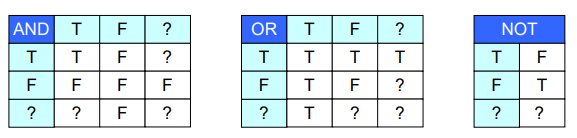
\includegraphics[width=0.7\textwidth]{tabella_verit_sql.png}
  \caption{Tabella di verità}
  \label{fig:tabella_verita-SQL}
\end{figure}
Per valutare gli attributi nulli è necessario usare IS NULL o IS NOT NULL.\\
\begin{itemize}
  \item IS NULL - vero se attributo ha valore nullo, falso altrimenti
  \item IS NOT NULL - vero se attributo ha valore specificato, falso altrimenti
\end{itemize}
\paragraph*{Esempio per la seguente tabella}
\begin{tabular}{|c|c|c|}
  \hline
  A & B & C \\
  \hline
  a & ? & c1 \\
  \hline
  a1 & b & c2 \\
  \hline
  a2 & ? & ? \\
  \hline
\end{tabular}
\begin{lstlisting}[language=SQL]
  SELECT *
  FROM Tabella
  WHERE B IS NULL
\end{lstlisting}
Restituisce t1 e t3.
\paragraph*{Esempio reali} Query: gli impiegati che \textbf{sono} o \textbf{potrebbero essere}
ingegneri.
\begin{lstlisting}[language=SQL]
  SELECT *
  FROM Impiegato
  WHERE mansione = 'Ingegnere' OR mansione IS NULL
\end{lstlisting}
\subsection{SELECT - DISTINCT}
In algebra relazionale i risultati della interrogazioni non contengono
elementi duplicati, mentre in SQL le tabelle prodotte dalle interrogazioni
possono contenere più righe identiche tra loro.\\
I duplicati possono essere rimossi usando la parola chiave DISTINCT.
\begin{lstlisting}[language=SQL]
  SELECT [DISTINCT] AttrEspr
  FROM Tabella
  [WHERE Condizione]
\end{lstlisting}
\subsection{Espressioni e Funzioni}
I predicati usati nelle interrogazioni possono coinvolgere, oltre a
nomi di colonna anche espressioni. Le espressioni sono formulate
applicando operatori ai valori delle colonne delle tuple.\\
Esempi di espressioni e funzioni sono que40lle aritmetiche su stringhe,
su date e tempi. Le espressioni possono comparire nelle clausole
SELECT, WHERE e UPDATE.
\paragraph*{SELECT} Una espressione usata nella clausola SELECT
dà luogo ad una nuova colonna che non corrisponde a nessuna colonna
della tabella su cui si effettua la selezione (argomento di FROM).\\
Questa colonna è detta Colonna \textbf{virtuale}. Le colonne virtuali non sono
fisicamente memorizzate, ma sono materializzate (esistono) solo come risultato
delle interrogazioni.\\
Anche alle colonne virtuali è possibile assegnare un alias (con il
costrutto AS).\\
\paragraph*{Funzioni predefinite}
\begin{itemize}
  \item su stringhe (UPPER, UCASE, LENGTH)
  \item su date, intervalli (+, -, DATE, DAYOFWEEK, ...)
  \item matematiche (*, +, -, /, TAN, SQRT, SIN, ...)
  \item informazioni di istema (USER, CURRENT\_DATE, ...) 
\end{itemize}
\paragraph*{Esempio} Trovare stipendio mensile degli impiegati che guadagnano
più di 40.\\
Dato che lo stipendio memorizzato nel DB è annuale, bisogna dividere per 12.
\begin{lstlisting}[language=SQL]
  SELECT stipendio/12 AS stipendio_mensile
  FROM Impiegato
  WHERE stipendio > 40
\end{lstlisting}
Se non inserisco un ALIAS la colonna virtuale avrà un nome generato (non significativo).
\paragraph*{Funzioni per le stringhe}
Gli operatori più comuni sono:
\begin{itemize}
  \item || - concatenazione
  \item UPPER, UCASE - Trasforma la stringa in caratteri maiuscoli
  \item LOWER, LCASE - Trasforma la stringa in caratteri minuscoli
\end{itemize}
\section{Operatore JOIN}
L'operatore JOIN rappresenta un'importante funzionalità in quanto
permette di correlare dati in tabelle diverse.\\
Matematicamente si tratta del prodotto cartesiano tra le due tabelle,
che avrà un numero di righe pari al prodotto del numero di righe
delle due tabelle e viene applicata una condizione di matching tra 
le colonne specificate. Il puro prodotto cartesiano avviene fra le
tabelle inserite nel FROM, mentre la condizione di matching è inserita
o nel WHERE (\textbf{JOIN implicito}) o nel FROM esplicitando il JOIN (\textbf{JOIN esplicito}).\\
Ad un operatore JOIN sono applicati uno o più predicati di join.\\
Un predicato di join esprime una condizione che deve essere verificata
dalle tuple del risultato dell'interrogazione.
Il predicat di join permette di estrarre dal DB un sottoninsieme opportuno
del prodotto cartesiano.
\subsection{JOIN implicito}
Quando la condizione di selezione viene inserita nel WHERE allora sto
effettuando un JOIN implicito.
\paragraph*{Esempio}
\begin{lstlisting}[language=SQL]
  SELECT *
  FROM Impiegato, Dip
  WHERE Impiegato.Dipart = Dip.Nome;
\end{lstlisting}
In questo caso ho estratto tutte le informazioni sugli impiegati e sui
dipartimenti in cui lavorano.\\
\paragraph*{Esempio Esami}
Estrarre Matricola, Cognome, Nome Voto di tutti gli studenti che
hanno sostenuto l'esame di 'Analisi I'.
\begin{lstlisting}[language=SQL]
  SELECT S.Matricola, S.Cognome, S.nome, E.Voto
  FROM Studenti AS S, Esami AS E
  WHERE (S.Matricola = E.Studente) AND (E.Corso = 'Analisi I')
\end{lstlisting}
Come già detto in precedenza il FROM efettua il prodotto cartesiano, mentre
la condizione di WHERE indica il predicato di join.\\
\subsection{JOIN esplicito}
Introdotto in SQL-2, è possibile effettuare esplicitamente il JOIN
nella clausola FROM
\begin{lstlisting}[language=SQL]
  SELECT AttrExpr [ [AS] Alias ] {, AttrExpr [[AS] Alias ] }
  FROM Tabella [ [AS] Alias ]
  { [ TipoJoin ] JOINTabella [[AS] Alias ] ONCondizJoin}
  [ WHERE CondizQuery ]
\end{lstlisting}
In questo modo esplicitiamo il JOIN sulle tabelle e separiamo
le condizioni di JOIN dalle condizioni di QUERY.
\paragraph*{Tipi di JOIN}
\begin{itemize}
  \item INNER (questo prefisso non si mette dato che è il JOIN di default)
  \item OUTER JOIN
  \begin{itemize}
    \item RIGTH [OUTER]
    \item LEFT [OUTER]
    \item FULL [OUTER]
  \end{itemize}
\end{itemize}
\paragraph*{Esempio JOIN sul seguente schema}
\begin{center}
  \begin{tabular}{|c|c|c|c|c|c|c|c|c|c|}
    \hline
    ID\_impiegato & Nome & Cognome & Dipart & Ufficio & Stipendio & premioprod & Mansione & Città & IDCapo \\
    \hline
  \end{tabular}
\end{center}
\begin{tabular}{|c|c|c|}
  \hline
  Nome & Indirizzo & Città\\
  \hline
\end{tabular}
\begin{lstlisting}[language=SQL]
  SELECT I.Nome, I.Cognome, Dip.Citta
  FROM Impiegato AS I JOIN Dip ON I.Dipart = Dip.Nome
\end{lstlisting}
Non si ha traccia delle tuple di impiegato che non corrispondono
ad alcuna tupla di Dip.
\subsection{OUTER JOIN}
L'operatore di OUTER JOIN aggiunge l risultato le tuple di Impiegato e Dip che non hanno partecipato al JOIN,
completandole con NULL.\\
Consideriamo il seguente esempio:
\begin{lstlisting}[language=SQL]
  FROM Impiegato AS I [FULL|LEFT|RIGHT] OUTER JOIN Dip ON ...
\end{lstlisting}
\paragraph*{LEFT} Le tuple di impiegato che non partecipano al join vengono completate ed inserite
nel risultato.
\paragraph*{RIGHT} Le tuple di Dip che non partecipano al join vengono completate ed inserite nel
risultato.
\paragraph*{FULL} (Sia Left che Right) Sia le tuple di impiegato che quelle di Dip che non partecipano al join
vengono completate ed inserite nel risultato.
\subsection{Self JOIN}
JOIN effettuato sulla stessa tabella.
\paragraph*{Esempio}
\begin{lstlisting}[language=SQL]
  SELECT G1.Genitore AS Nonno
  FROM Genitori G1, Genitori G2
  WHERE G1.Figlio = G2.Genitore
  AND G2.Figlio = 'Anna'
\end{lstlisting}
In questo caso vengono ricercati i nonni di Anna. \'E possibile fare questo perchè
quando seleziono le tabelle nel FROM tratto delle loro copie, quindi posso anche prenderle due volte.
\section{Operatori di ordinamento e aggregazione}
\subsection{Ordinamento del risultato: ORDER BY}
Le righe sono ordinate in base al primo attributo, se i valori sono uguali,
viene ordinata in base al secondo attributo ecc.\\
Ordinamento: ascendente (ASC), discendente (DESC), (ASC è default e può
essere omesso).
\paragraph*{Esempio}
\begin{lstlisting}[language=SQL]
  SELECT *
  FROM Impiegato
  ORDER BY Stipendio
\end{lstlisting}
L'opzione DESC è relativa al singolo attributo, quindi va specificata per ciascun attributo
che elenco nell'ORDER BY.\\
\subsection{Operatori aggregazione}
Sono un'estensione rispetto all'Algebra Relazionale. Essi operano su gruppi di tuple per:
\begin{itemize}
  \item Effettuare calcoli sull'insieme di tuple
  \item Verificare condizioni relative all'insieme di tuple
\end{itemize}
\begin{itemize}
  \item COUNT - Conta numero di tuple di tabella
  \item SUM - Somma valori o espressioni di attributi
  \item MAX - Valore massimo di un attributo di tabella
  \item MIN - Valore minimo di un attributo di tabella
  \item AVG - Valore medio di un attributo di tabella
  \item GROUP BY - Raggruppamento delle tuple in sottogruppi gestiti come estensione
  delle normali interrogazioni
\end{itemize}
\paragraph*{Come vengono applicati}
\begin{itemize}
  \item Si esegue l'interrogazione sulla base di clausole FROM e WHERE.
  \item Si applica l'operatore aggregato alla tabella risultato dell'interrogazione.
\end{itemize}
\subsection{COUNT}
\begin{lstlisting}[language=SQL]
  SELECT COUNT(< * | [DISTINCT | ALL] ListaAttr >)
\end{lstlisting}
\begin{itemize}
  \item DISTINCT numero di valori distinti diversi da NULL di ListaAttr
  \item ALL numero di valori diversi da NULL di ListaAttr
  \item COUNT (*) conta numero di righe di una tabella
\end{itemize}
Se non è specificato nulla, ALL è l'opzione di default.
\paragraph*{Esempio} Estrarre il numero di impiegati del dipartimento Produzione
\begin{lstlisting}[language=SQL]
  SELECT COUNT(*) AS impiegati_produzione
  FROM Impiegato
  WHERE dipart='Produzione'
\end{lstlisting}
L'operatore aggregato COUNT viene applicato al risultato dell'interrogazione.\\
\paragraph*{COUNT e valori nulli}
COUNT(*) conta anche le righe con valori NULL, dato che conta le righe totali della tabella.\\
COUNT(Attributo) non conta le righe NULL.\\
COUNT(DISTINCT Attributo) non conta le righe NULL e non conta i valori duplicati.
\subsection{Altri operatori di aggregazione}
\begin{lstlisting}[language=SQL]
  < SUM | MAX | MIN | AVG > (< * | [DISTINCT | ALL] AttrExpr >)
\end{lstlisting}
Valutano espressioni analizzando tuple del risultato nella query che li contiene. Operano
su tuple di tabella prese come insieme di elementi (non su elementi individuali).
DISTINCT e ALL si applicano come per il caso di COUNT.
\paragraph*{SUM} Restituisce la somma dei valori di AttrExpr relativamente alle tuple di tabella specificate
nella query. Opera su attributi numerici.
\paragraph*{MIN MAX} Restituisce il minimo/massimo dei valori di AttrExpr relativamente alle tuple di tabella 
specificate nella query. Opera su atributi ordinabili (stringhe, numer, ecc.).\\
\paragraph*{AVG} Restituisce la media dei valori di AttrExpr relativamente alle tuple di tabella specificate, opera
su valori numerici.
\subsection{Operatori di aggregazione e Target List}
SQL impedisce di includere in una stessa target list funzioni aggregate e espressioni al livello
di riga.
\paragraph*{Esempio}
\begin{lstlisting}[language=SQL]
  SELECT Cognome, MAX(Stipendio) -- ERRORE
  FROM Impiegato
  WHERE Dipart = 'Amministrazione'
\end{lstlisting}
La soluzione è effettuare una query nidificata (spiegata in seguito).
\begin{lstlisting}[language=SQL]
  SELECT Cognome, Stipendio
  FROM Impiegato
  WHERE Dipart = 'Amministrazione'
  AND Stipendio = (SELECT MAX(I1.Stipendio) 
                  FROM Impiegato AS I1
                  WHERE I1.Dipart = 'Amministrazione')
\end{lstlisting}
\subsection{GROUP BY}
La clausola GROUP BY serve a definire gruppi omogenei di tuple, specificando una o
più colonne (di raggruppamento) sulla base della/e quale/i le tuple sono raggruppate
per valori uguali.\\
\paragraph*{Esempio}
Data la seguente tabella estrarre la somma degli stipendi degli impiegati che afferiscono
allo stesso dipartimento.
\begin{figure}[h]
  \centering
  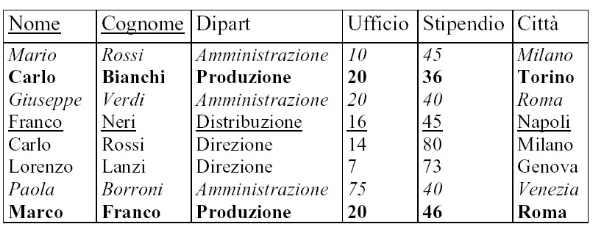
\includegraphics[width=0.7\textwidth]{es_group_by.png}
  \caption{Tabella esercizio}
  \label{fig:tabella_es_groupby}
\end{figure}
\begin{lstlisting}[language=SQL]
  SELECT Dipart, SUM(Stipendio)
  FROM Impiegato
  GROUP BY Dipart
\end{lstlisting}
Come viene eseguita la query? Analizziamola passo per passo:
\paragraph*{Esecuzione senza GROUP BY}
In questo caso mi restituisce tutti gli attributi della SELECT in un'unica tabella.\\
Con GROUP BY invece vengono raggruppate le righe del risultato come specificato
nel GROUP BY (nell'esempio valori Dipart).
\begin{figure}[h]
  \centering
  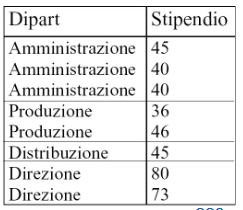
\includegraphics[width=0.3\textwidth]{tabella_groupby.png}
  \caption{Tabella con GROUP BY}
  \label{fig:tabella_groupby}
\end{figure}
\paragraph*{Applicazione SUM dopo GROUP BY} 
Così facendo l'applicazione dell'operatore SUM avviene su gruppi di tuple con lo stesso nome.
\begin{table}[h]
  \centering
  \begin{tabular}{|c|c|}
    \hline
    Dipart & sum(Stipendio) \\
    \hline
    Amministrazione & 125 \\
    \hline
    Produzione & 82 \\
    \hline
    Distribuzione & 45\\
    \hline
    Direzione & 153 \\
    \hline
  \end{tabular}
  \caption{Tabella somma stipendi per dipartimento}
  \label{tabella_stipendi}
\end{table}
\newpage
Il GROUP BY raggruppa sempre gli gli attributi specificati nella clausola GROUP BY con lo stesso
nome, permettendo poi di applicare condizioni particolari nella SELECT (per esempio AVG, COUNT, ecc.).
\subsection{Raggruppamenti e Target List}
\paragraph*{Importante restrizione} Una clausola di proiezione di una query contenente la clausola
GROUP BY può solo includere:
\begin{enumerate}
  \item Una o più colonne se compaiono nella clausola GROUP BY
  \item Operatori di aggregazione (COUNT, SUM, AVG, ...)
\end{enumerate}
Nella SELECT deve apparire l'attributo specificato nel GROUP BY, altrimenti la Query risulterà
scorretta.
\begin{lstlisting}[language=SQL]
  SELECT nome, cognome -- nome e' ERRORE!
  FROM persone
  GROUP BY cognome

  SELECT cognome, AVG(Eta) -- Corretta
  FROM persone
  GROUP BY cognome
\end{lstlisting}
Tutti gli attributi nella SELECT devono essere sepcificati anche nel GROUP BY.
\subsection{Condizioni sui Gruppi}
Verificano condizioni su gruppi di tuple aggregate con GROUP BY.
\begin{itemize}
  \item WHERE - Verifica condizioni su tuple individuali
  \item HAVING - Verifica condizioni (espressioni booleane) su gruppi di tuple
  (opera su raggruppamenti)
\end{itemize}
Le condizioni in clausola HAVING sono verificate dopo la creazione dei sottogruppi
di tuple specificati da GROUP BY.\\
\paragraph*{Esempio}
Trovare i dipartimenti che spendono più di 100 in stipendi.
\begin{lstlisting}[language=SQL]
  SELECT Dipart, SUM(Stipendio) AS SommaStipendi
  FROM Impiegato
  GROUP BY Dipart
  HAVING SommaStipendi > 100
\end{lstlisting}
\paragraph*{Risolviamo la Query passo per passo.}
\begin{enumerate}
  \item Esecuzione della query senza considerare GROUP BY e operatori
  aggregati
  \item Raggruppamento delle righe del risultato come specificato da GROUP BY
  \item Applicazione dell'operatore di aggregazione SUM su Stipendio ai gruppi di
  righe precedentemente costruiti
  \item Selezione dei gruppi risultanti come specificato dalla clausola HAVING
\end{enumerate}
Qui vediamo proprio la differenza di HAVING rispetto a WHERE, dato che
WHERE opera su tuple individuali (selezione di tuple prima di GROUP BY),
mentre HAVING opera su predicati che operano su gruppi di tuple creati da
GROUP BY (selezone raggruppamenti).
\paragraph*{Esempio molto utile} Andare alla slide N 247 (62 come Pagina PDF)
delle slide del prof \href{https://elearning.unimib.it/pluginfile.php/1533829/mod_resource/content/1/SQL.pdf}{Slide Prof}.
\subsection{Osservazioni}
\begin{lstlisting}[language=SQL]
  GROUP BY attr1, attr2
  -- Equivalente a
  GROUP BY attr2, attr1
\end{lstlisting}
\paragraph*{HAVING osservazioni}
La sintassi permette di definire la clausola HAVING anche senza la clausola GROUP BY.
In questo caso l'intero insieme di righe è trattato come un unico raggruppamento, è
necessario ricordarsi che per HAVING devono essere usati solo predicati in cui
compaiono operatori aggregati.
\section{Interrogazioni di tipo insiemistico}
Permettono di costruire query concatenando due query SQL
\begin{itemize}
  \item UNION
  \item INTERSECT
  \item EXCEPT (differenza)
\end{itemize}
\paragraph*{Sintassi}
\begin{lstlisting}[language=SQL]
  SelectSQL { < UNION/INTERSECT/EXCEPT > [ALL] SelectSQL }
\end{lstlisting}
I duplicati vengono eliminati (a meno che si usi ALL).
\subsection{UNION}
Restituisce tutte le tuple distinte restituire da almeno una delle sottointerrogazioni a qui
è applicata.\\
L'operatore UNION elimina i duplicati dal risultato, mentre UNION ALL li mantiene.\\
UNION impone alcune importanti restrizioni sulle interrogazioni su cui opera:
\begin{itemize}
  \item Le interrogazioni devono restituire lo stesso numero di colonne, e le colonne corrispondenti devono avere
  lo stesso dominio (non è richiesto che abbiano la stessa lunghezza) o domini compatibili
  \item La corrispondenza si basa sulla posizione delle colonne, indipendentemente dal loro nome
  \item Se si usa la clausola ORDER BY questa deve essere usata una sola volta alla
  fine dell'interrogazione e non alla fine di ogni SELECT
\end{itemize}
\subsection{INTERSECT, EXCEPT, MINUS}
\begin{itemize}
  \item L'operatore INTERSECT esegue l'intersezione
  \item Gli operatori EXCEPT e MINUS eseguono la differenza
\end{itemize}
Per questi operatori valgono le stesse condizioni di applicabilità viste per l'operatore
UNION. Le interrogazioni devono restituire lo stesso numero di clonne e le colonne corrispondenti
devono avere lo stesso dominio (non è richiesto che abbiano la stessa lunghezza) o domini compatibili.
La corrispondenza si basa sulla posizione delle colonne.\\

\section{Interrogazioni nidificate}
Una delle ragioni che rendono SQL un linguaggio potente è la possibilità di esprimere
interrogazioni più complesse in termini di interrogazioni più semplici, tramite il
meccanismo delle \textbf{subqueries} (sottointerrogazioni).\\
La clausola WHERE di una query (detta query esterna) può infatti contenere un'altra
query (detta subquery).\\
La subquery viene usata per determinare uno o più valori da usare come valori di confronto
in un predicato della query esterna.\\
Nella clausola WHERE possono comparire predicati che confrontano un attributo (o un'espressione
sugli attributi) con il risultato di una query SQL:
\paragraph*{Sintassi}
\begin{lstlisting}[language=SQL]
  ScalarValue Operator <ANY | ALL > SelectSQL
\end{lstlisting}
\begin{itemize}
  \item ANY - Il predicato è vero se almeno una riga restituita dalla query SelectSQL 
  soddisfa il confronto
  \item ALL - Il predicato è vero se tutte le righe restituite dalla query SelectSQL soddisfano il
  confronto
  \item Operator - Uno qualsiasi tra $=, <>, >, <, >=, <=$
\end{itemize}
La query che appare nella clausola WHERE è detta \textbf{query nidificata}.\\
\paragraph*{Esempio} Estrarre il cognome degli impiegati che lavorano in dipartimenti con
sede a Milano.\\
\textit(IN = ANY).
\begin{lstlisting}[language=SQL]
  SELECT Cognome
  FROM Impiegato
  WHERE dipart ANY (SELECT nome
                    FROM Dip
                    WHERE Citta = 'Milano')

  -- Equivale a

  SELECT cognome
  FROM Impiegato JOIN Dip
    ON dip.Nome = impiegato.Dipart
    WHERE Dip.Citta = 'Milano'
\end{lstlisting}
La forma ndificata è meno dichiarativa, ma talvolta  più leggibile (richiede meno variabili).
La forma piana e quella nidificata possono essere combinate.
\paragraph*{Osservazione} Le sottointerrogazioni non possono contenere operatori insiemistici (si fanno
solo a livello esterno), la limitazione non è significativa.
\subsection{Operatori di confronto}
Gli operatori di confronto $=, <$, ... si possono usare solo se la subquery restituisce
non più di una tupla (detta subquery "scalare").\\
Se la subquery può restituire più di un valore allora si devono usare le forme:
\begin{itemize}
  \item ANY - la relazione = vale per almeno uno dei valori
  \item ALL - la relazione $>$ vale per tutti i valori
\end{itemize}
Ricordiamo che la forma ANY = IN.
\subsection{MAX e MIN in subquery}
Gli operatori aggregati max e min possono essere usati in una subquery.\\
Anche in questo caso è necessario usare ANY o ALL se vengono restituiti più valori:
\begin{itemize}
  \item ANY la relazione vale per aleno uno dei valori
  \item ALL la relazione vale per tutti i valori
\end{itemize}
% Slide 295 - 74